% !Mode:: "TeX:UTF-8"
%!TEX program  = xelatex

\documentclass[bwprint,fontset=windows]{gmcmthesis}

\hypersetup{hidelinks}
\usepackage[framemethod=TikZ]{mdframed}

%\usepackage{fontspec}  % for Consolas & Courier New
%\lstset{basicstyle=\small\fontspec{Consolas}}
%\lstset{basicstyle=\small\fontspec{Courier New}}
%\setmonofont{Consolas}
%\setcounter{tocdepth}{3}   % 调整目录深度

\usepackage{subfig}
\usepackage{colortbl}
\definecolor{color1}{rgb}{0.78,0.88,0.99}
\definecolor{color2}{rgb}{0.36,0.62,0.84}
%\definecolor{color3}{rgb}{0.8235,0.8706,0.9373}
\definecolor{color3}{rgb}{0.88,0.92,0.96}
\definecolor{color4}{rgb}{0.96,0.97,0.98}%{0.9176,0.9373,0.9686}

% 算法
\usepackage[noend]{algpseudocode}
\usepackage{algorithmicx,algorithm}
\floatname{algorithm}{算法}
\renewcommand{\algorithmicrequire}{\textbf{输入:}}
\renewcommand{\algorithmicensure}{\textbf{输出:}}

%\numberwithin{equation}{section}
%\numberwithin{figure}{section}
%\numberwithin{table}{section}


\newcommand{\red}[1]{\textcolor{red}{#1}}
\newcommand{\blue}[1]{\textcolor{blue}{#1}}


%===================== 建模论文题目 ======================

\title{全国研究生数学建模竞赛论文标题}
\baominghao{\hspace{6em} 20230900001} %参赛队号
\schoolname{\hspace{5.8em} 学校名称填写} %学校名称
\membera{\hspace{6em} 成员A} %队员A
\memberb{\hspace{6em} 成员B} %队员B
\memberc{\hspace{6em} 成员C} %队员C

%=======================================================


\begin{document}

 %生成标题
 \maketitle

 %填写摘要
\begin{abstract}
本模板是为全国研究生数学建模竞赛编写的 \LaTeX{} 模板, 旨在让大家专注于
论文的内容写作, 而不用花费过多精力在格式的定制和调整上. 本手册是相应的参考, 其
中提供了一些环境和命令可以让模板的使用更为方便. 同时需要注意, 使用者需要有一
定的 \LaTeX{} 的使用经验, 至少要会使用 ctex 宏包的一些功能, 比如调节字距或修改字体
大小等等.

 \begin{mdframed} [%
	roundcorner=5pt,
	linecolor=gray!50,
	outerlinewidth=0.5pt,
	middlelinewidth=0.3pt, backgroundcolor=gray!2,
innertopmargin=\topskip, frametitle={2024年格式变化说明},
frametitlefont= \bfseries,frametitlerule=true,frametitlealignment =\raggedright\noindent,
frametitlerulewidth=.5pt, frametitlebackgroundcolor=gray!2,]
今年的格式变化如下:
\begin{enumerate}
\item 论文第一页为标识替换;
\item 合并 \url
{https://github.com/andy123t/GMCMthesis} 更新. 修复首页页码;
\item 调整摘要、标题、关键词和浮动体标题等字体。
\end{enumerate}

\end{mdframed}

这是研究生报名官方网站,点击\href{https://cpipc.chinadegrees.cn}{\fbox{这里}}进入。

欢迎大家到QQ群里沟通交流:91940767/478023327/640633524。我们也开通了问答区交流 \LaTeX{}技术:\url{https://ask.latexstudio.net},欢迎大家前来交流。


\keywords{折叠桌\quad  曲线拟合\quad   非线性优化模型\quad  受力分析}

\end{abstract}

\pagestyle{plain}

%目录 不推荐加
\maketoc

\clearpage

\section{在线使用}

如果你想要在 Overleaf 使用, 那么需要设置下字体
\begin{lstlisting}[language={[latex]TeX}]
\documentclass[bwprint,fontset=fandol]{gmcmthesis}
\end{lstlisting}

由于线上平台没有隶书,只能用楷体替代了, 大家根据自己的情况来使用。



\uwave{欢迎关注我们的微信公众号}:

\centerline{
\includegraphics[width=5cm]{gongzhonghao1}}

\section{问题重述}

 
在保持原题主体思想不变下,可以自己组织词句对问题进行描述,主要数据可以直接复制,对所提出的问题部分基本原样复制。篇幅建议不要超过一页。
\section{问题分析}
主要是表达对题目的理解,特别是对附件的数据进行必要分析、描述(一般都有数据附件),这是需要提到分析数据的方法、理由。如果有多个小问题,可以对每个小问题进行分别分析。
(假设有2个问题)



\subsection{问题1的分析}

对问题1研究的意义的分析。

问题1属于。。。。。数学问题,对于解决此类问题一般数学方法的分析。

对附件中所给数据特点的分析。

对问题1所要求的结果进行分析。

由于以上原因,我们可以将首先建立一个。。。。。。的数学模型I,然后将建立一个。。。。。。。的模型II,。。。。。。。。。。对结果分别进行预测,并将结果进行比较.


\subsection{问题2的分析}


对问题2研究的意义的分析。



\section{模型假设}

1.	假设题目所给的数据真实可靠;

2.

3.
 
 

 注意:假设对整篇文章具有指导性,有时决定问题的难易。一定要注意假设的某种角度上的合理性,不能乱编,完全偏离事实或与题目要求相抵触。注意罗列要工整。
 
\section{定义与符号说明}
(对文章中所用到的主要数学符号进行解释)

。。。。。。。。。。。。。。。。。。。。。。。。。。。。。。。。。。。。。。。。。。。

尽可能借鉴参考书上通常采用的符号,不宜自己乱定义符号,对于改进的一些模型,符号可以适当自
己修正(下标、上标、参数等可以变,主符号最好与经典模型符号靠近)。对文章自
己创新的名词需要特别解释。其他符号要进行说明,注意罗列要工整。
注意格式统一,不要出现零乱或前后不一致现象,关键是容易看懂。


\section{符号说明}


\begin{table}[htp!]
\centering
\renewcommand\arraystretch{1.2} %定义表格高度
\newcolumntype{L}{>{\quad}X}
\newcolumntype{P}[1]{>{\centering\arraybackslash}p{#1}}
\newcolumntype{C}{>{\centering \arraybackslash}X}
\newcolumntype{R}{>{\raggedright \arraybackslash}X}
\begin{tabularx}{0.9\textwidth}{!{\color{color2}\vrule}P{2cm}!{\color{color2}\vrule}L!{\color{color2}\vrule}}
  \arrayrulecolor{color2}\hline %\toprule
  \rowcolor{color2}
  \textbf{符号}    &   \quad \textbf{意义} \\
  \arrayrulecolor{color2}\hline %\midrule
  %\rowcolor[gray]{0.90}
  \rowcolor{color3}
  $ a $  &  符号1的意义    \\
  \arrayrulecolor{color2}\hline
  \rowcolor{color4}
  $ b $  &  符号2的意义    \\
  \arrayrulecolor{color2}\hline
  \rowcolor{color3}
  $ c $  &  符号3的意义符号3的意义    \\
  \arrayrulecolor{color2}\hline
  \rowcolor{color4}
  $ d $  &  符号4的意义    \\
  \arrayrulecolor{color2}\hline
  \rowcolor{color3}
  $ e $  &  符号5的意义     \\
  \arrayrulecolor{color2}\hline
  \rowcolor{color4}
  $ f $  &  符号6的意义符号6的意义    \\
  \arrayrulecolor{color2}\hline
  \rowcolor{color3}
  $ g $  &  符号7的意义     \\
  \arrayrulecolor{color2}\hline
  \rowcolor{color4}
  $ h $  &  符号8的意义     \\
  \arrayrulecolor{color2}\hline
  \rowcolor{color3}
  $ i $  &  符号9的意义符号9的意义     \\
  \arrayrulecolor{color2}\hline
  \rowcolor{color4}
  $ k $  &  符号10的意义     \\
  \arrayrulecolor{color2}\hline
\end{tabularx}
\end{table}

%\begin{tabularx}{\textwidth-18pt}{XXX}
%\hline
%Input & Output& Action return \\
%\hline
%DNF &  simulation & jsp\\
%\hline
%\end{tabularx}


\section{模型的建立}

\subsection{问题一分析}
题目要求建立模型描述折叠桌的动态变化图,由于在折叠时用力大小的不同,我们不能描述在某一时刻折叠桌的具体形态,但我们可以用每根木条的角度变化来描述折叠桌的动态变化。首先,我们知道折叠桌前后左右对称,我们可以运用几何知识求出四分之一木条的角度变化。最后,根据初始时刻和最终形态两种状态求出桌腿木条开槽的长度


\subsection{算法示例}

数学建模求解算法示例:
\begin{center}
\begin{minipage}{0.8\textwidth}
\begin{algorithm}[H]%[!htp]
\caption{算法的名字} %算法的名字
{\bf 输入:} %算法的输入, \hspace*{0.02in}用来控制位置,同时利用 \\ 进行换行
input parameters A, B, C\\
{\bf 输出:} %算法的结果输出
output result
\begin{algorithmic}[1]
\State some description 算法介绍 % \State 后写一般语句
\For{condition} % For 语句,需要和EndFor对应
  \State ...
  \If{condition} % If 语句,需要和EndIf对应
    \State ...
  \Else
    \State ...
  \EndIf
\EndFor
\While{condition} % While语句,需要和EndWhile对应
  \State ...
\EndWhile
\State \Return result
\end{algorithmic}
\end{algorithm}
\end{minipage}
\end{center}
\vspace{2ex}

\section{表格和图形}

\subsection{表格}

%\begin{table}[!htbp]
%    \caption{标准三线表格}\label{tab:001} \centering
%    \begin{tabular}{ccccc}
%        \toprule%[1.5pt]
%        $D$(in) & $P_u$(lbs) & $u_u$(in) & $\beta$ & $G_f$(psi.in)\\
%        \midrule%[1pt]
%        5 & 269.8 & 0.000674 & 1.79 & 0.04089\\
%        10 & 421.0 & 0.001035 & 3.59 & 0.04089\\
%        20 & 640.2 & 0.001565 & 7.18 & 0.04089\\
%        \bottomrule%[1.5pt]
%    \end{tabular}
%\end{table}

三线表
\begin{table}[!htp]
\newcolumntype{L}{X}
\newcolumntype{C}{>{\centering \arraybackslash}X}
\newcolumntype{R}{>{\raggedright \arraybackslash}X}
\centering
\caption{某校学生升高体重样本}
\label{tab2:heightweight}
\begin{tabularx}{0.9\textwidth}{CCCC}
   \toprule
	序号&年龄&身高&体重\\
	\midrule
	1&14&156&42\\
	2&16&158&45\\
	3&14&162&48\\
	4&15&163&50\\
    \midrule
    %\cmidrule{2-4}
	平均&15&159.75&46.25\\
	\bottomrule
\end{tabularx}
\end{table}

模型建立的思路想好之后,采取了怎样的算法对模型进行了实现。前面建了几个模型,这里就有几个模型的求解。(如利用Matlab编程求解、用spss软件求解,利用拉普拉斯变换求解,用蒙特卡罗模拟求解等。特别是求解有难度的模型要介绍求解方法。)获得什么样的结果,可围绕题目要求综合给出关键结论,建议不要将问题所需结果全部给出,否则摘要显得太长。
 

模型建立的思路想好之后,采取了怎样的算法对模型进行了实现。前面建了几个模型,这里就有几个模型的求解。(如利用Matlab编程求解、用spss软件求解,利用拉普拉斯变换求解,用蒙特卡罗模拟求解等。特别是求解有难度的模型要介绍求解方法。)获得什么样的结果,可围绕题目要求综合给出关键结论,建议不要将问题所需结果全部给出,否则摘要显得太长。
 


模型建立的思路想好之后,采取了怎样的算法对模型进行了实现。前面建了几个模型,这里就有几个模型的求解。(如利用Matlab编程求解、用spss软件求解,利用拉普拉斯变换求解,用蒙特卡罗模拟求解等。特别是求解有难度的模型要介绍求解方法。)获得什么样的结果,可围绕题目要求综合给出关键结论,建议不要将问题所需结果全部给出,否则摘要显得太长。
 
某行业产量与生产费用的数据
\begin{table}[htp!]
\centering
\caption{某行业产量与生产费用的数据}%\label{}
\newcolumntype{Y}{>{\centering\arraybackslash}X}
\newcolumntype{Z}{!{\vline}@{\color{white}\vrule width \doublerulesep}!{\vrule}}%自定义列格式(双线)
\begin{tabularx}{0.94\textwidth}{c|c|YZc|c|Y}\Xhline{0.9pt}
	企业编号&	产量(台)&生产费用(万元)&企业编号&产量(台)&生产费用(万元)\\\Xcline{1-3}{0.6pt}\Xcline{4-6}{0.6pt}
	1&	40&	130&7&	84&	165\\
	2&	42&	150&8&	100&	170\\
	3&	50&	155&9&	116&	167\\
	4&	55&	140&10&	125&	180\\
	5&	65&	150&11&	130&	175\\
	6&	78&	154&12&	140&	185\\\Xhline{0.72pt}
\end{tabularx}
\end{table}

研究生数学建模2019年F题结果示例
\begin{table}[htp!]
\centering
\caption{问题1结果1 (左) 与 问题2结果 (右)}
\begin{minipage}[h]{0.48\linewidth}
\renewcommand\arraystretch{1.2} %定义表格高度
\newcolumntype{Y}{>{\centering\arraybackslash}X}
\begin{tabularx}{0.9\textwidth}{|Y|Y|Y|}
  \hline
  \rowcolor{color1}
  数据集1  &  数据集1 & 数据集2  \\
 \hline
  \rowcolor[gray]{0.95}
  A问题1   & A问题1 &  A问题1     \\
  \hline
  \rowcolor[gray]{0.9}
  503   &  503     & 163     \\
  \rowcolor[gray]{0.95}
  294   &  200     & 114      \\
  \rowcolor[gray]{0.9}
  91    &  80      & 8     \\
  \rowcolor[gray]{0.95}
  607   &  237     & 309      \\
  \rowcolor[gray]{0.9}
  540   &  170     & 305    \\
  \rowcolor[gray]{0.95}
  250   &  278     & 123    \\
  \rowcolor[gray]{0.9}
  340   &  369     & 45      \\
  \rowcolor[gray]{0.95}
  277   &  214     & 160    \\
  \rowcolor[gray]{0.9}
  B     &  397     & 92    \\
  \rowcolor[gray]{0.95}
        &  B       & 93    \\
  \rowcolor[gray]{0.9}
        &          & 61        \\
  \rowcolor[gray]{0.95}
        &          & 292       \\
  \rowcolor[gray]{0.9}
        &          & B         \\
  \rowcolor[gray]{0.95}
104861  & 103518   & 109342 \\
\hline
\end{tabularx}
\end{minipage}
\begin{minipage}[h]{0.48\linewidth}
\renewcommand\arraystretch{1.2} %定义表格高度
\newcolumntype{Y}{>{\centering\arraybackslash}X}
\begin{tabularx}{0.9\textwidth}{|Y|Y|Y|}
  \hline
  \rowcolor{color1}
  数据集1  &  数据集1 & 数据集2  \\
  \hline
  \rowcolor[gray]{0.95}
  A问题2  &  A问题2  & A问题2    \\
  \hline
  \rowcolor[gray]{0.9}
   503    & 503     & 163  \\
  \rowcolor[gray]{0.95}
  294    & 200     & 114   \\
  \rowcolor[gray]{0.9}
   91     & 80     & 8   \\
  \rowcolor[gray]{0.95}
   607    & 237     & 309   \\
  \rowcolor[gray]{0.9}
   540    & 170    & 305  \\
  \rowcolor[gray]{0.95}
   250    & 278    & 123  \\
  \rowcolor[gray]{0.9}
   340    & 369     & 45   \\
  \rowcolor[gray]{0.95}
   277    & 214    & 160  \\
  \rowcolor[gray]{0.9}
  B      & 397   & 92 \\
  \rowcolor[gray]{0.95}
        &  B     &  93      \\
  \rowcolor[gray]{0.9}
         &         &  61      \\
  \rowcolor[gray]{0.95}
        &         &   292     \\
  \rowcolor[gray]{0.9}
        &         &   B     \\
  \rowcolor[gray]{0.95}
 104917  &  103563  &109427 \\
\hline
\end{tabularx}
\end{minipage}
\end{table}

\clearpage
\begin{table}[htp!]
%\small
\centering
\renewcommand\arraystretch{1.2} %定义表格高度
\newcolumntype{Y}{>{\centering\arraybackslash}X}
\caption{问题3结果}
\begin{tabularx}{0.9\textwidth}{|Y|Y|Y|Y|Y|Y|}
\hline %定义表格宽度
\rowcolor{color1}
  数据集1  &  数据集1  &  \multicolumn{2}{c|}{数据集2 (无问题点)}  & \multicolumn{2}{c|}{数据集2 (有问题点)} \\
\hline
\rowcolor[gray]{0.95}
  A问题3   & A问题3   &  \multicolumn{2}{c|}{A问题3}    &  \multicolumn{2}{c|}{A问题3}      \\
  \hline
  \rowcolor[gray]{0.9}
  503      & 503     & 169      & 73      & 169     & 73   \\
  \rowcolor[gray]{0.95}
  69       & 69      & 322      & 249     & 322     & 249   \\
  \rowcolor[gray]{0.9}
  506      & 506      & 270     & 274     & 270     & 274   \\
  \rowcolor[gray]{0.95}
  371      & 371      & 89      & 12      & 89      & 12   \\
  \rowcolor[gray]{0.9}
  183      & 183      & 236     & 216     & 236     & 216  \\
  \rowcolor[gray]{0.95}
  194      & 194      & 132     & 16      & 132     & 16   \\
  \rowcolor[gray]{0.9}
  450      & 450      & 53      & 282     & 53      & 282   \\
  \rowcolor[gray]{0.95}
  286      & 113      & 112     & 84      & 112     & 141  \\
  \rowcolor[gray]{0.9}
  485      & 485      &  268    & 287     & 268     & 291 \\
  \rowcolor[gray]{0.95}
 \red{B (9D)}~~     & 248      & 250     & 99      & 250     &161 \\
 \rowcolor[gray]{0.9}
   & \red{B (10D)}   & 243     & \red{B (21D)}   & 243    & \red{B (21D)} \\
 \rowcolor[gray]{0.95}
    &          &         &         &         &       \\
 \rowcolor[gray]{0.9}
  104861m  & 103518m  &         & 168924m  &         &161650m \\
\hline
\end{tabularx}
\end{table}



\subsection{图形}

图形并列
\begin{figure}[htp!]
\begin{minipage}[t]{0.48\linewidth}
\centering
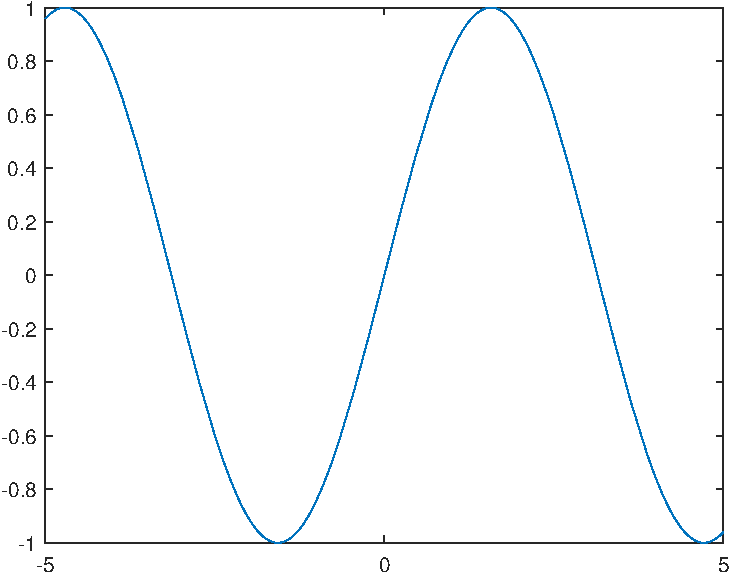
\includegraphics[width=0.9\textwidth]{image1}
\caption{fig1}
\label{fig:side:a}
\end{minipage}%
\begin{minipage}[t]{0.48\linewidth}
\centering
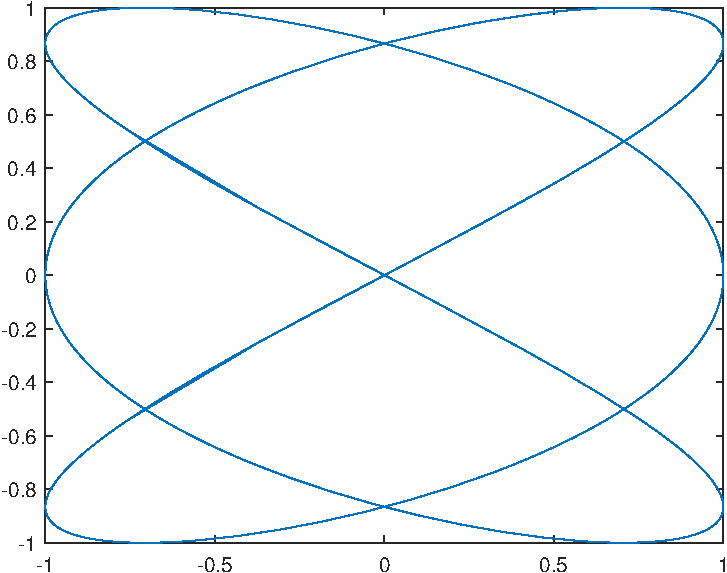
\includegraphics[width=0.9\textwidth]{image2}  % 2.2in
\caption{fig2}
\label{fig:side:b}
\end{minipage}
\end{figure}


\clearpage
这是一个算法流程图
\begin{figure}[htp!]
\centering
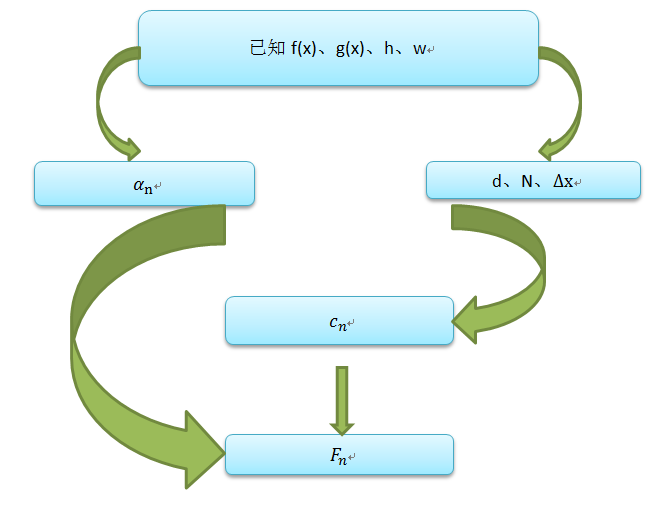
\includegraphics[width=.55\textwidth]{fig.png}
\caption{算法流程图}
\end{figure}

多图并排
\begin{figure}[!htp]
	\centering
	\subfloat[Arabic numerals]{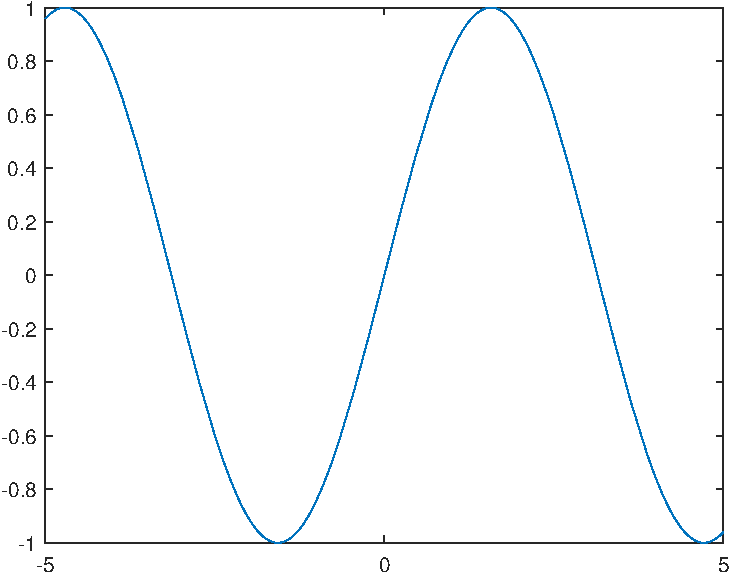
\includegraphics[width=0.4\textwidth]{image1}}\qquad
	\subfloat[Arabic numerals]{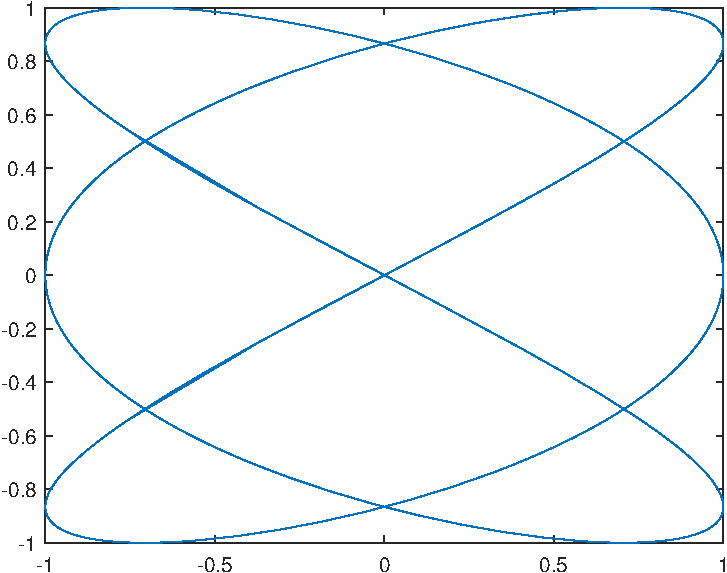
\includegraphics[width=0.4\textwidth]{image2}} \\
	\subfloat[Arabic numerals]{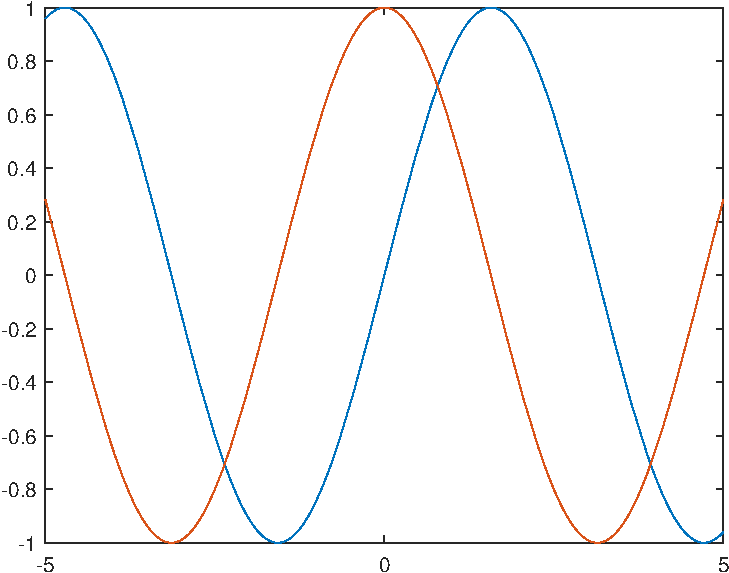
\includegraphics[width=0.4\textwidth]{image3}}\qquad
	\subfloat[Arabic numerals]{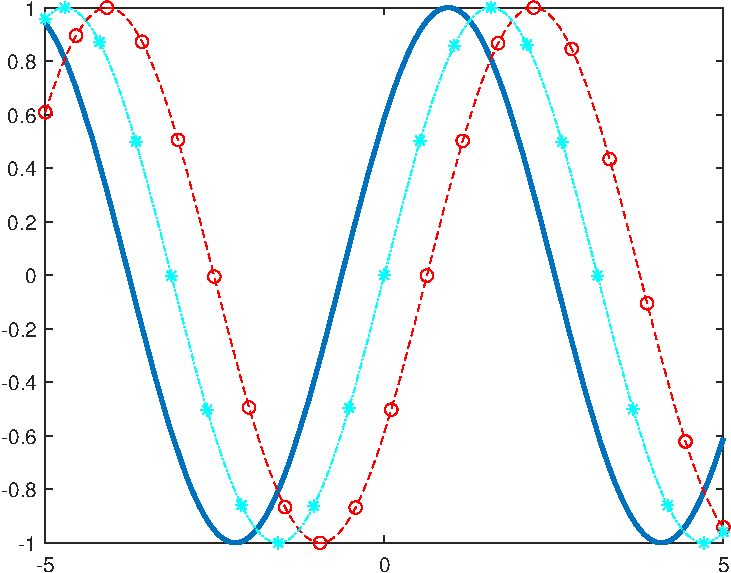
\includegraphics[width=0.4\textwidth]{image4}}
	\caption{多图示例}
\end{figure}


\subsection{问题三分析}


题目要求制作软件的意思就是客户给定折叠桌高度、桌面边缘线的形状大小和桌脚边缘线的大致形状,将这些信息输入程序就得到客户想要的桌子。我们在求解最优设计加工参数时,自行给定桌面边缘线形状(椭圆、相交圆等),桌脚边缘线形状,折叠桌高度,应用第二问的非线性规划模型,用MATLAB软件绘制折叠桌截面图,得到自己设计的创意平板折叠桌。


\section{模型评价}

这里是模型评价



%参考文献   手工录入
%\begin{thebibliography}{9}%宽度9
% \bibitem{bib:one} ....
% \bibitem{bib:two} ....
%\end{thebibliography}

%采用bibtex方案
\cite{mittelbach_latex_2004,wright_latex3_2009,beeton_unicode_2008,vieth_experiences_2009,ls:2024}

\bibliographystyle{gmcm}
\bibliography{reference}


\clearpage
%附录
\begin{appendices}
%\setcounter{page}{1} %如果需要可以自行重置页码。
\section{MATLAB 源程序}
\renewcommand{\thesubsection}{A\thinskip.\thinskip\arabic{subsection}}
\subsection{第1问程序}
\vspace{-2ex}

\begin{Matlab}{code.m}
clear all
kk=2;
[mdd,ndd]=size(dd);
while ~isempty(V)
    [tmpd,j]=min(W(i,V));
    tmpj=V(j);
    for k=2:ndd
        [tmp1,jj]=min(dd(1,k)+W(dd(2,k),V));
        tmp2=V(jj);
        tt(k-1,:)=[tmp1,tmp2,jj];
    end
    tmp=[tmpd,tmpj,j;tt];
    [tmp3,tmp4]=min(tmp(:,1));
    if tmp3==tmpd,
        ss(1:2,kk)=[i;tmp(tmp4,2)];
    else
        tmp5=find(ss(:,tmp4)~=0);
        tmp6=length(tmp5);
        if dd(2,tmp4)==ss(tmp6,tmp4)
            ss(1:tmp6+1,kk)=[ss(tmp5,tmp4);tmp(tmp4,2)];
        else, ss(1:3,kk)=[i;dd(2,tmp4);tmp(tmp4,2)];
        end
    end
    dd=[dd,[tmp3;tmp(tmp4,2)]];
    V(tmp(tmp4,3))=[];
    [mdd,ndd]=size(dd);kk=kk+1;
end;
S=ss; D=dd(1,:);
\end{Matlab}
\vspace{2ex}

\clearpage
\section{Python 源程序}
\renewcommand{\thesubsection}{B\thinskip.\thinskip\arabic{subsection}}
\subsection{第2问程序}
\vspace{-2ex}
\begin{Python}{mip1.py}
# This example formulates and solves the following  MIP model:
#  maximize
#        x +   y + 2 z
#  subject to
#        x + 2 y + 3 z <= 4
#        x +   y       >= 1
#        x, y, z binary

# import gurobipy as gp
from gurobipy import * #GRB
try:
    # Create a new model
    m = Model("mip1")
    # Create variables
    x = m.addVar(vtype=GRB.BINARY, name="x")
    y = m.addVar(vtype=GRB.BINARY, name="y")
    z = m.addVar(vtype=GRB.BINARY, name="z")
    # Set objective
    m.setObjective(x + y + 2 * z, GRB.MAXIMIZE)
    # Add constraint: x + 2 y + 3 z <= 4
    m.addConstr(x + 2 * y + 3 * z <= 4, "c0")
    # Add constraint: x + y >= 1
    m.addConstr(x + y >= 1, "c1")
    # Optimize model
    m.optimize()
    for v in m.getVars():
        print('%s %g' % (v.varName, v.x))
    print('Obj: %g' % m.objVal)

except GurobiError as e:
    print('Error code ' + str(e.errno) + ': ' + str(e))

except AttributeError:
    print('Encountered an attribute error')
\end{Python}

\end{appendices}



\end{document}
